\chapter{Étude d'un prédicteur de Smith}
Nous allons maintenant passer à l'analyse d'un autre type de correction de systèmes à retard : le prédicteur de Smith. Ce type de correcteur permet d'établir une commande de système retardé en utilisant une estimation du procédé qui sera utilisé en temps $t$ et $t+h$.

\section{Schéma de principe du prédicteur de Smith}
Nous avons dessiné avec \emph{Simulink} le schéma bloc en figure \ref{fig:sch_predicteurSmith}, dans lequel nous avons séparé $\tilde{C}(p)$ (C\_Smith sur le schéma) et  $ G(p) e ^{-hp}$(Procédé dans le schéma).
\begin{figure}[!ht]
\centering
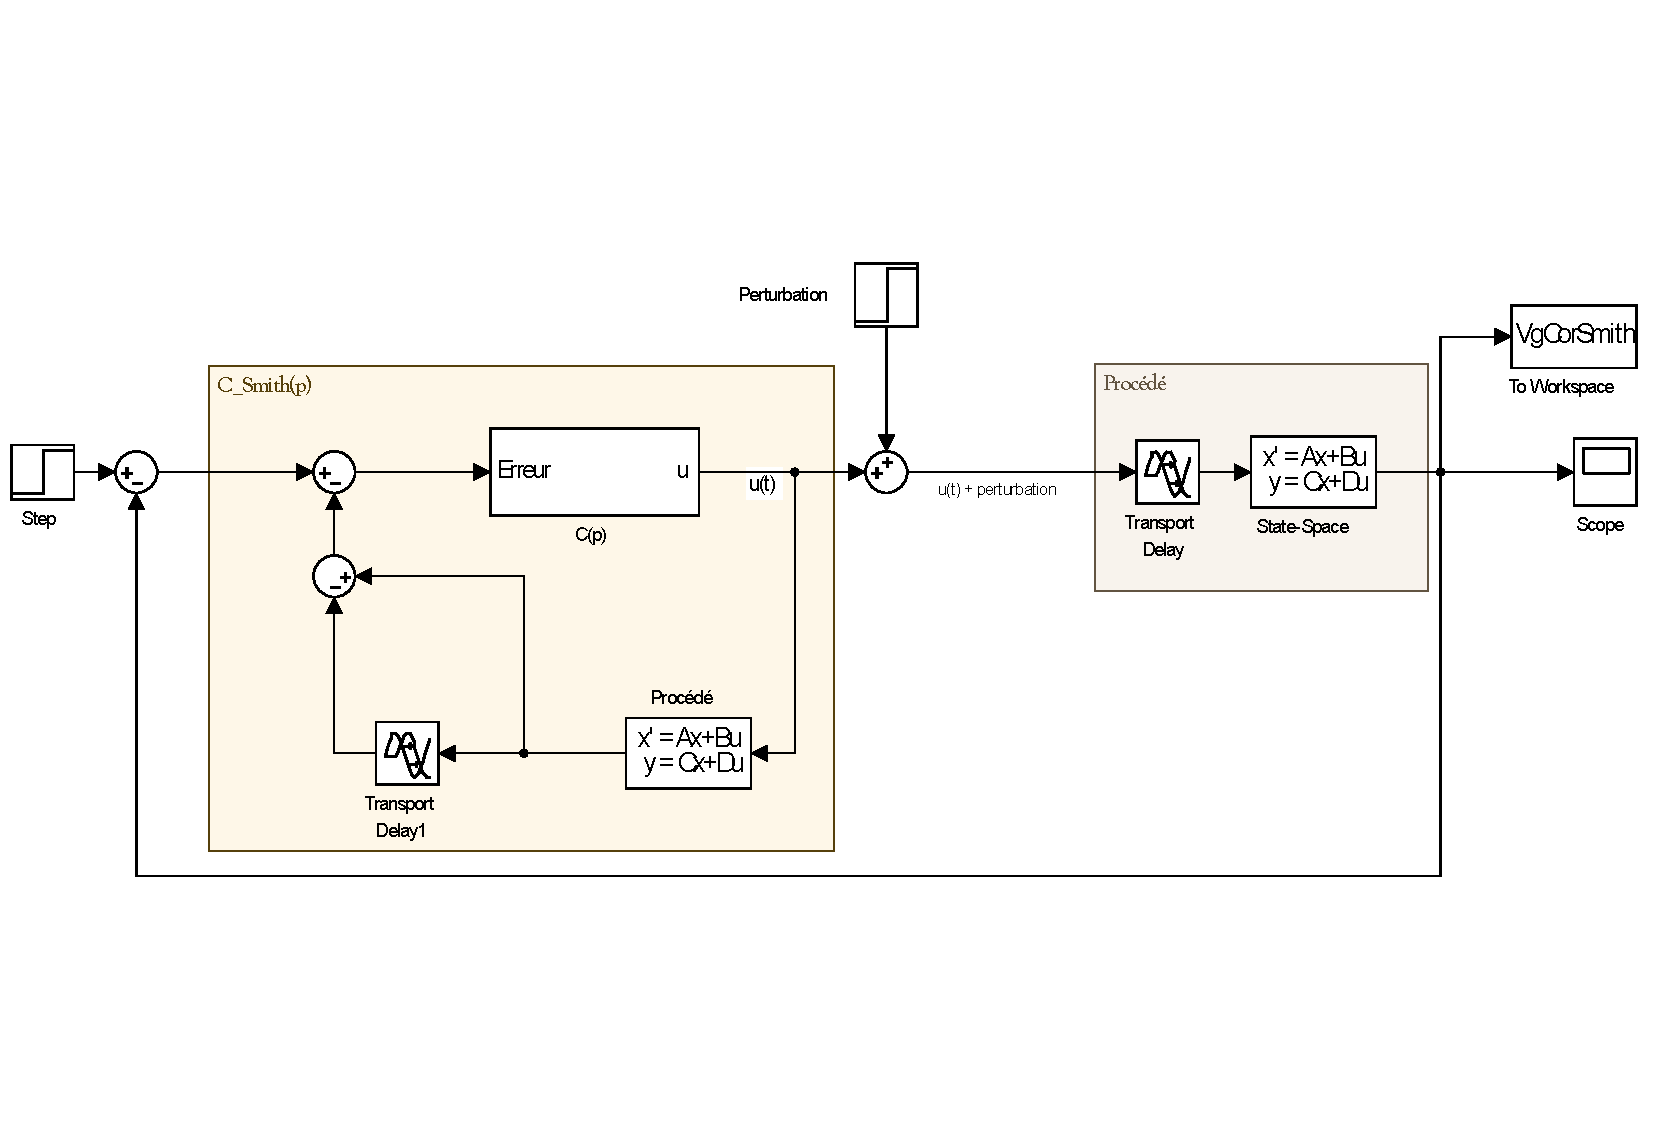
\includegraphics[width=\textwidth]{./IV/images/schema_Predicteur.pdf}
\caption{Schéma de principe du prédicteur de Smith}\label{fig:sch_predicteurSmith}
\end{figure}
Le bloc $C(p)$ devra contenir le bloc de commande que nous souhaitons utiliser. Il pourra être complexe ou bien plus simple.

\section{Fonction de transfert du système en boucle fermé}
Pour obtenir le transfert en boucle fermé de ce schéma, nous allons nous référencer à des résultats de cours et TD, qui sont : 
\begin{equation}
\tilde{C}(p) = \frac{C(p)}{1+G(p)\left(1-e^{-hp}\right)}C(p)	
\end{equation}
ainsi que le transfert de boucle fermé qui s'écrit :
\begin{align}
G_{bf} &= \frac{\tilde{C}G(p)e^{-hp}}{1+\tilde{C}G(p)e^{-hp}}\\
	   &= \frac{C(p)G(p)e^{-hp}}{1+G(p)C(p)}	
\end{align}

Nous utiliserons cette fonction de transfert pour déterminer, à partir du correcteur établi dans les prochaines parties, le polynôme caractéristique du système. 

\section{Correcteur sur le prédicteur de Smith}
On nous propose de mettre un correcteur simple dans la bloc $C(p)$, celui ci sera de a forme : $C(p) = k_0$, soit, un correcteur proportionnel. Nous obtenons avec ce nouvel élément, la fonction de transfert enboucle fermé suivante :
\begin{equation}
G_{bf}(p) = \frac{k_sk_rk_me^{-hp}}{\tau p +p+k_0k_sk_rk_m}
\end{equation}
L'analyse du polynôme caractéristique vient alors dans les équations suivantes :
\begin{align*}
\tau p + p + k_0k_sk_rk_m = 0 \Leftrightarrow p_{1,2} = \frac{-1 \pm \sqrt{1-4\tau k_0k_sk_rk_m}}{2\tau}
\end{align*}
Plusieurs conditions apparaissent alors sur le gain proportionnel pour assurer le cahier des charges : \begin{itemize}
\item [\textbullet]$Re(p_{1,2}) < 0$ pour assurer la stabilité. De cette hypothèse, nous avons alors forcement :\begin{equation}
1-4\tau k_0k_sk_rk_m < 1 \Leftrightarrow k_0 > 0
\end{equation}
Résultat logique, bien qu'il existe des correcteurs avec un gain admis de manière négative, nous sommes ici dans un cas trivial qui n'admet qu'un gain proportionnel positif.
\item [\textbullet] $1-4\tau k_0k_sk_rk_m \geq 0$ pour ne pas avoir des pôles complexes conjugués. Nous avons alors :
\begin{equation}
4\tau k_0k_sk_rk_m \leq 1 \Leftrightarrow k_0 \leq \frac{1}{4\tau k_sk_rk_m}
\end{equation}
\paragraph*{Valeur du Correcteur $C(p)$} \underline{Application numérique} Nous avons alors un correcteur qui est : \begin{equation}\label{eqn:corPredicteurSmith}
C(p) = 0.0925
\end{equation}
\end{itemize}